\documentclass{beamer}
\usetheme{Malmoe}
\usecolortheme{beetle}
%\usepackage[left=2cm, right=2cm, top=3cm]{geometry}
\usepackage[utf8]{inputenc}
%\usepackage{amsmath}
\usepackage{mathtools,amssymb,amsfonts}
\usepackage{hyperref}
\usepackage{graphicx,float}
\usepackage{tikz}
\usetikzlibrary{shapes.geometric, arrows}

\title{Part-of-Speech Tagging with Word Embeddings}
\subtitle{CS 9875 Final Project}
\author{Paul Moore \and Juhani Dickinson}
\date{\today}

%Copied from Stackexchange at https://tex.stackexchange.com/a/178803
\AtBeginSection[]{
	\begin{frame}
	\vfill
	\centeringn
	\begin{beamercolorbox}[sep=8pt,center,shadow=true,rounded=true]{title}
		\usebeamerfont{title}\secname\par%
	\end{beamercolorbox}
	\vfill
	\end{frame}
}

\makeatletter
\patchcmd{\beamer@section}{{#2}{\the\c@page}}{{#1}{\the\c@page}}{}{}
\makeatother

\begin{document}

\begin{frame}
	\titlepage
\end{frame}

\begin{frame}
	\frametitle{Outline}
	\tableofcontents
\end{frame}

\section[Section shortname]{Section 1 Longname}
\subsection*{Subsection 1}
\begin{frame}
	\frametitle{Slide Title}
	Slide text
\end{frame}
\begin{frame}
	\frametitle{Slide Title 2}
	\begin{center}
	Slide text 2
	\end{center}
\end{frame}
\subsection*{Subsection 2}
\begin{frame}
	Slide text
\end{frame}

%https://tex.stackexchange.com/questions/699195/how-to-use-texorpdfstring-correctly-and-properly
\subsection*{Subsection 3}
\begin{frame}
	\frametitle{Slide Title}
	Slide text
\end{frame}



%NOTE Paul's Section

\section[Word Embedding Models]{Word Embedding Models}

\begin{frame}\centering
  \frametitle{What are word embeddings?}
  % https://assets.zilliz.com/Figure_Word_Embeddings_b021a5a759.png
  
  \includegraphics[width=0.75\linewidth]{assets/word-embedding-example.png}
  %TODO citation
\end{frame}

\subsection*{Static Word Embeddings}

\begin{frame}
  \frametitle{Static Word Embeddings}
  What are static word embedding models?
\end{frame}

\begin{frame}\centering
  \frametitle{Word2Vec}
  \begin{columns}
    \begin{column}{.4\linewidth}\centering
      \includegraphics[width=\linewidth]{assets/cbow.png}\par 
      CBOW
    \end{column}

    \begin{column}{.4\linewidth}\centering
      \includegraphics[width=\linewidth]{assets/skipgram.png}\par 
      Skip Gram
    \end{column}
\end{columns} %TODO citation
\bigskip
Word2Vec Training Procedures
\end{frame}

\begin{frame}
  \frametitle{Word2Vec}
  \[\begin{bmatrix}
    W_{00} & W_{01} & W_{02} & ...\\
    W_{10} & W_{11} & W_{12} & ...\\
    W_{20} & W_{21} & W_{22} & ...\\
    ... & ... & ... & ... 
  \end{bmatrix}\]
\end{frame}

\subsection*{Contextual Word Embeddings}

\begin{frame}
  \frametitle{Contextual Word Embeddings}\centering
  What are contextual word embeddings?
\end{frame}


% https://deeplobe.ai/wp-content/uploads/2021/04/1.jpg
% https://learnopencv.com/wp-content/uploads/2023/10/bert-masked-language-modeling-1.png


\begin{frame}\centering
  \frametitle{BERT}
  \begin{columns}
  \begin{column}{.4\linewidth}\centering
    \includegraphics[width=\linewidth]{assets/transformer.png}\par
    Transformer architecture
  \end{column}

  \begin{column}{.4\linewidth}\centering
    \includegraphics[width=\linewidth]{assets/mlm.png}\par
    MLM
  \end{column}

  
 \end{columns} 
 %TODO citation  
\end{frame}


\begin{frame}\centering
  \frametitle{BERT}
  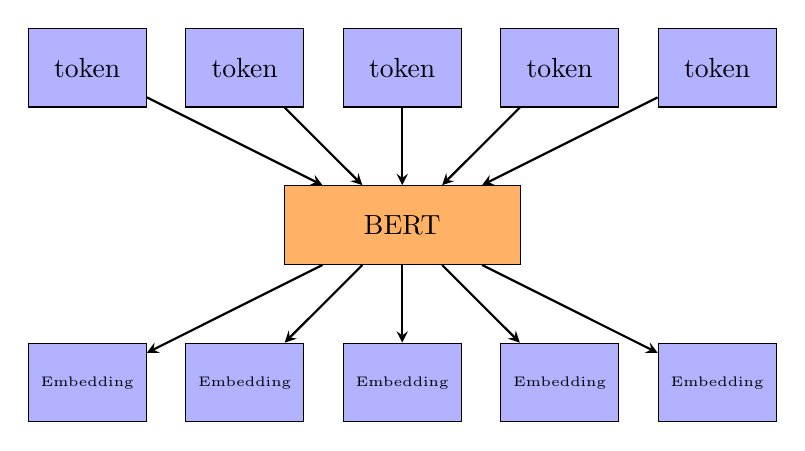
\begin{tikzpicture}
    \tikzstyle{io} = [rectangle, minimum width=1.5cm, minimum height=1cm, text centered, draw=black, fill=blue!30]
\tikzstyle{bert} = [rectangle, minimum width=3cm, minimum height=1cm, text centered, draw=black, fill=orange!60]
\tikzstyle{arrow} = [thick,->,>=stealth]
    \node (in1) [io] {token};
    
\node (in2) [io, right of=in1, xshift=1cm] {token};
\node (in3) [io, right of=in2, xshift=1cm ]{token};
\node (in4) [io, right of=in3, xshift=1cm ] {token};
\node (in5) [io, right of=in4, xshift=1cm ] {token};
\node (bert) [bert, below of=in3, yshift=-1cm ] {BERT};
\node (out1) [io, below of=bert, yshift=-1cm, xshift=-4cm] {\tiny Embedding};
\node (out2) [io, below of=bert, yshift=-1cm, xshift=-2cm] {\tiny Embedding};
\node (out3) [io, below of=bert, yshift=-1cm] {\tiny Embedding};
\node (out4) [io, below of=bert, yshift=-1cm, xshift=2cm] {\tiny Embedding};
\node (out5) [io, below of=bert, yshift=-1cm, xshift=4cm] {\tiny Embedding};

\draw[arrow] (in1) -- (bert);
\draw[arrow] (in2) -- (bert);
\draw[arrow] (in3) -- (bert);
\draw[arrow] (in4) -- (bert);
\draw[arrow] (in5) -- (bert);

  \draw [arrow] (bert) -- (out1);
\draw [arrow] (bert) -- (out2);
\draw [arrow] (bert) -- (out3);
\draw [arrow] (bert) -- (out4);
\draw [arrow] (bert) -- (out5);
  \end{tikzpicture}
\end{frame}

\begin{frame}
  
\end{frame}

\end{document}
